\begin{Problem}
\begin{parts}
	\item Benutzen Sie Proposition 5.6.9, um zu zeigen, dass
		\[
		g(x)=\sin(x)\cosh(x), \qquad x\in \R
		\] 
durch die zugehörige Taylorreihe im Punkt $x_0 = 0$ mit Konvergenzradius $R=+\infty$ dargestellt wird.
\item Zeigen Sie, dass $f:\R\to \R$ mit
	\[
	f(x)=\begin{cases}
		\exp\left( -\frac{1}{x^2} \right) & \qquad x \neq 0\\
		0 & \text{sonst}
	\end{cases}
	\]
	\emph{nicht} durch ihre Taylorreihe um x = 0 dargestellt wird. Warum ist dies kein Widerspruch zu Proposition 5.6.9?
\end{parts}	
\end{Problem}
\begin{proof}
	\begin{parts}
	\item \begin{align*}
			g(x)=&\sin(x)\cosh(x)\\
			=&\left( \frac{e^{ix}-e^{-ix}}{2i} \right) \left( \frac{e^x+e^{-x}}{2} \right) \\
			=& \frac{1}{4i}\left( e^{(i+1)x}+e^{(i-1)x}-e^{(1-i)x}-e^{-(i+1)x} \right)\\
			=& \frac{i}{4}\left[ e^{-(i+1)x}+e^{(1-i)x}-e^{(i+1)x}-e^{(i-1)x} \right]\\
			g^{(n)}(x)=&\frac{i}{4}\left[ \left[ -(i+1) \right]^n e^{-(i+1)x}+(1-i)^n e^{(1-i)x}\right.\\
 &\left.-(1+i)^n e^{(i+1)x}-(i-1)^n e^{(i-1)x} \right]\\
			|g^{(n)}(x)|\le& \frac{1}{4}(\sqrt{2})^n\left[ \left| e^{-(i+1)x} \right| +\left| e^{(1-i)x} \right| +\left| e^{(i+1)x} \right| +\left| e^{(i-1)x} \right|   \right] 
		\end{align*}
		Die Bedingungen sind jetzt erfüllt: Sei $B_r(0)^{cl}$ ein abgeschlossenes Ball für beliebige $r>0$. Sei außerdem
\begin{gather*}
			c=\sup_{x\in B_r(0)^{cl}}\frac{1}{4}\left[ \left| e^{-(i+1)x} \right| +\left| e^{(1-i)x} \right| +\left| e^{(i+1)x} \right| +\left| e^{(i-1)x} \right|   \right]\\
			\alpha=\sqrt{2} 
\end{gather*}
Es gilt $c\neq \infty$, weil die Abbildung in den Klammern stetig ist, und ist daher auf eine eingeschränkte Menge auch eingeschränkt. Es folgt:
\begin{equation}\tag{5.6.23}
	\|g^{(n)}\|_{B_r(0)^{cl}}\le c\alpha^n
\end{equation}
Also die formale Taylorreihe hat einen Konvergenzradius $R>r$ und konvergiert gegen auf $B_r(0)^{cl}$ gegen $g$. Weil das f\"{u}r alle $r>0$ gilt, konvergiert die Taylorreihe gegen $f$ f\"{u}r alle $x\in \R$, und die Konvergenzradius $R=+\infty$.
\item Es ist klar, dass es nicht durch ihre Taylorreihe dargestellt wird. Die Taylorreihe ist $0+0x+0x^2+\dots=0$, aber $f(x)\neq 0$ f\"{u}r $x\neq 0$.

	Wir berechnen jetzt $f^{(n)}(a)$. Es gilt
	\begin{align*}
		f(a)=&\exp(-1 / a^2)\\
		f'(x)=&\frac{2}{x^2}\exp(-1 / x^2)\\
		f''(x)=&\left[ \frac{4}{x^6}-\frac{6}{x^4} \right]\exp(-1 / x^2)\\
		f'''(x)=&\left[ \frac{8}{x^9}-\frac{36}{x^7}+\frac{24}{x^5} \right]\exp(-1 / x^2) \qedhere
	\end{align*}
	Aber das Supremum ist nicht nur durch die Koeffizienten beeinflusst, sondern auch das Maximumpunkt\ldots
	\begin{center}
		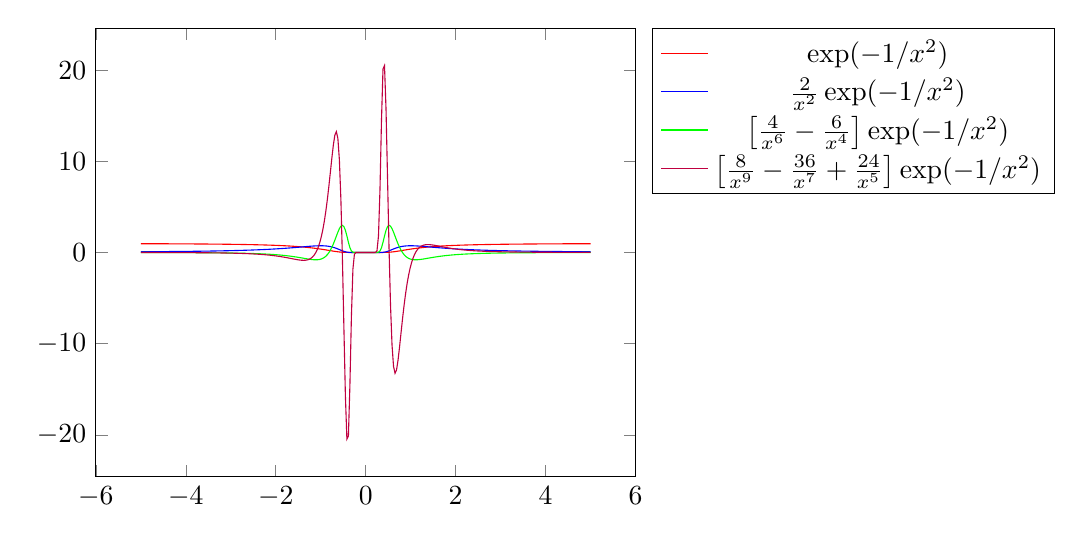
\begin{tikzpicture}
			\begin{axis}[samples=300,legend entries={$\exp(-1 / x^2)$,$\frac{2}{x^2}\exp(-1 / x^2)$,$\left[ \frac{4}{x^6}-\frac{6}{x^4} \right]\exp(-1 / x^2)$,$\left[ \frac{8}{x^9}-\frac{36}{x^7}+\frac{24}{x^5} \right]\exp(-1 / x^2) $},legend pos=outer north east]
				\addplot[domain=-5:5,color=red] {exp(-1 / x^2)};
				\addplot[domain=-5:5,color=blue] {2/x^2*(exp(-1/x^2))};
				\addplot[domain=-5:5,color=green] {(4/x^6-6/x^4)*exp(-1/x^2)};
				\addplot[domain=-5:5,color=purple] {(8/x^9-36/x^7+24/x^5)*exp(-1/x^2)};
			\end{axis}
		\end{tikzpicture}
	\end{center}
	Also
	\begin{center}
		\includegraphics[width=0.2\textwidth]{gg.png}
	\end{center}
	\end{parts}
\end{proof}
\begin{Problem}
	Es sei $f : \R_0^+ \to \R$ definiert durch $f (x) = \sqrt[3]{x}$. Geben Sie das Taylorpolynom $P_2$ von f mit Entwicklungspunkt $x_0 = 1$ an und schätzen Sie den maximalen Fehler von $|f(x) - P_2(x)|$ auf dem Intervall $\left[ \frac{1}{2},\frac{3}{2} \right] $ ab.
\end{Problem}
\begin{proof}
	Es gilt $f(x)=x^{1 / 3}$, und daher
	\[
		f^{(n)}(x)=\left[\prod_{i=0}^{n-1} \left( \frac{1}{3}-i \right) \right]x^{\frac{1}{3}-n} 
	,\] 
	also
	\[
		f^{(n)}(1)=\prod_{i=1}^{n-1} \left( \frac{1}{3}-i \right)  
	.\] 
	Es gilt daher
	\[
	P_2(x)=1+\frac{1}{3}(x-1)-\frac{1}{9}(x-1)^2
	.\] 
	Wir wissen schon
	\begin{equation}\tag{5.6.20}
		\left| R_{n,x_0}(f)(h) \right| \le \sup_{t\in[0,1]}\left| f^{(n)}(x_0+th)-f^{(n)}(x_0) \right| \frac{|h|^n}{(n-1)!}
	\end{equation}
	Hier ist $n=2$, und $|h|\le \frac{1}{2}$. 
\begin{tcolorbox}[title=Vereinfachung]
	(Nur in diesem Problem, falsch im Allgemein) Der maximale Fehler ist gleich $\sup_{t\in [-1,1]}\left| f^{(n)}(x_0+th)-f^{(n)}(x_0) \right| \frac{|h|^n}{(n-1)!}$, wobei $h=\frac{1}{2},n=2$, und $x_0=1$.
\begin{proof}
	Wir betrachten zuerst $R_{n,x_0}(f)(\xi)$ f\"{u}r $0\le\xi\le h$. Es gilt
	\begin{align*}
		\sup_{\xi\in [0,h]}R_{n,x_0}(f)(\xi)\le& \sup_{\xi\in [0,h]}\left[\sup_{t\in [0,1]}\left| f^{(n)}(x_0+t\xi)-f^{(n)}(x_0) \right| \frac{|\xi|^n}{(n-1)!}\right]\\
		=& \sup_{\xi\in [0,h]}\left[\sup_{t\in [0,1]}\left| f^{(n)}(x_0+t\xi)-f^{(n)}(x_0) \right| \frac{|h|^n}{(n-1)!} \right] \\
		=&\sup_{t\in [0,1]}\left| f^{(n)}(x_0+th)-f^{(n)}(x_0) \right| \frac{|h|^n}{(n-1)!}
	\end{align*}
	Ähnlich gilt auch
	\[
		\sup_{\xi\in[-h,0]}R_{n,x_0}(f)(\xi)=\sup_{t\in [-1,0]}\left| f^{(n)}(x_0+th)-f^{(n)}(x_0) \right| \frac{|h|^n}{(n-1)!}
	.\] 
	Weil wir den maximalen Fehler auf dem ganzen Intervall schätzen möchten, ist die gewünschte Antwort daher
	\[
		\sup_{\xi\in[-h,h]}R_{n,x_0}(f)(\xi)=\sup_{t\in[-1,1]}\left| f^{(n)}(x_0+th)-f^{(n)}(x_0) \right| \frac{|h|^n}{(n-1)!}
	.\qedhere\] 
\end{proof}
\end{tcolorbox}
Wir betrachten deswegen
\begin{align*}
	&\sup_{t\in [-1,1]}\left| f^{(n)}(x_0+th)-f^{(n)}(x_0) \right|\\
	&= \sup_{t\in [-1,1]}\left| \left[\prod_{i=0}^{n-1}\left( \frac{1}{3}-i \right) \right] \left( x_0+th \right) ^{\frac{1}{3}-n}-\left[ \prod_{i=0}^{n-1}\left( \frac{1}{3}-i \right)    \right]    \right|\\
	&= \left| \prod_{i=0}^{n-1}\left( \frac{1}{3}-i \right) \right|\sup_{t\in[-1,1]}\left| \left(1+\frac{t}{2}\right)^{- 5 / 3}-1 \right| \\
	&=\left| \prod_{i=0}^{n-1} \left( \frac{1}{3}-i \right)  \right|\left| \left( 1-\frac{1}{2} \right)^{- 5 / 3}-1 \right|\\
	&=\left| \prod_{i=0}^{n-1}\left( \frac{1}{3}-i \right) \right| \left( 2^{5 / 3}-1 \right)  
\end{align*}
Also der maximale Fehler ist
\[
	\underbrace{\frac{1}{4}}_{|0.5|^2}\left| \prod_{i=0}^{n-1} \left( \frac{1}{3}-i \right)   \right| \left( 2^{5 / 3}-1 \right)=\frac{1}{18}\left( 2^{5 / 3}-1 \right)  
.\qedhere\]
\end{proof}
\begin{Problem}
	Bestimmen Sie die Taylorpolynome vom Grad 30 der folgenden Funktionen in $x_0$.
	\begin{parts}
	\item $f(x)=x^3-3x^2+3x+2$ im Punkt $x_0=2$.
	\item $g(x)=\sin^2\left( \pi x \right) $ in $x_0=3$.
	\item $h(x)=\sin^{-1}(x)$ in $x_0=0$.
	\end{parts}
\end{Problem}
\begin{proof}
	\begin{parts}
	\item 
		{\allowdisplaybreaks
		\begin{align*}
			f(2)=&2^3-3(2)^2+3(2)+2=4\\
			f'(x)=&3x^2-6x+3\\
			f'(2)=&3\\
			f''(x)=&6x-6\\
			f''(2)=&6\\
			f'''(x)=&6=f(2)\\
			f''''(x)=&0
		\end{align*}
	}
		Das Taylorpolynom ist dann
		\[
		4+3(x-2)+3(x-2)^2+(x-2)^3
		.\] 
	\item {\allowdisplaybreaks
		\begin{align*}
			g(x)=&\sin^2(\pi x)=\frac{1}{2}\left( 1-\cos(2\pi x) \right) \\
			g(3)=&0\\
			g'(x)=&\pi \sin(2\pi x)\\
			g^{(n)}(x)=&\left( -1 \right)^{\left\lfloor (n-1) / 2 \right\rfloor}\frac{(2\pi)^{n}}{2}\begin{cases}
				\sin(2\pi x) & n\text{ ungerade}\\
				\cos(2\pi x) & n\text{ gerade}
			\end{cases} & n\geq 1\\
				g^{(n)}(3)=& \left( -1 \right) ^{\left\lfloor (n - 1) / 2 \right\rfloor}\frac{(2\pi)^n}{2}\begin{cases}
					0 & n\text{ ungerade}\\
					1 & n\text{ gerade}	
				\end{cases} & n \ge 1
		\end{align*}
	}
		Das Taylorpolynom vom Grad 30 ist
		\[
			\sum_{n=1}^{15}\left[ \left( -1 \right) ^{\left\lfloor (2n -1) / 2 \right\rfloor}\frac{(2\pi)^{2n}}{2(2n)!}(x-3)^{2n}\right]
		.\] 
	\item
		{\allowdisplaybreaks
		\begin{align*}
			h(x)=& \sin^{-1}x\\
			h(0)=&0\\
			h'(x)=&\frac{1}{\sqrt{1-x^2} }=(1-x^2)^{-1 / 2}\\
			h'(0)=&1\\
		\end{align*}
		Sei $p(x)=\frac{1}{\sqrt{1-x^2} }$. Wir wissen, dass die Taylorreihe von $(1+x)^\alpha$
		\begin{equation}\tag{5.6.41}
			\sum_{n=0}^{\infty} \binom{\alpha}{n}x^n
		\end{equation}
		ist, wobei $\binom{\alpha}{n}=\frac{1}{n!}\left[ \alpha(\alpha-1)\dots(\alpha-n+1) \right] $. Die Taylorreihe von $\frac{1}{\sqrt{1-x^2} }$ folgt:
		\begin{align*}
			T_{0}\left( \frac{1}{\sqrt{1-x^2} } \right)(x)=& \sum_{n=0}^{\infty} \binom{-1 / 2}{n}\left( -x^2 \right)^n\\
			=& \sum_{n=0}^{\infty} \binom{-1 / 2}{n}(-1)^n(x^{2n})\\
			=& \sum_{n=0}^{\infty} b_n x_n & b_n=0\text{, n ungerade}
\end{align*}
		Es gilt daher, f\"{u}r die Koeffizienten der Taylorreihe von $\sin^{-1}(x)$
		 \[
			 T_{0}(\sin^{-1}(x))(x)=\sum_{n=0}^{\infty} a_n x^n
		,\] 
		dass $a_n=b_{n-1} / n$, f\"{u}r $n\ge 1$. Es ist dann
		 \[
			 T_{0}(\sin^{-1}(x))(x)=\sum_{n=0}^{14} \frac{1}{2n+1}\binom{-1 / 2}{n}(-1)^n(x^{2n+1})
		.\qedhere\] 
	}
	\end{parts}
\end{proof}
\begin{Problem}
	Bestimmen Sie die Ober- und Untersummen von $\exp : [0, 1] \to\R$ für die markierten Zerlegungen $(J_n, \Xi_n)$ mit der Auswahl $\Xi_n = \left\{ 0,\frac{1}{n},\frac{1}{n},\dots,\frac{n-1}{n},1 \right\} $ für $n \in \N$. Zeigen Sie anschließend, dass die zugehörigen Ober- und Untersummen gegen denselben Wert konvergieren.
\end{Problem}

\begin{proof}\noindent 
	\begin{tcolorbox}[breakable]
		Wir werden später die folgende Lemma brauchen:
	\begin{Lemma}
		\[\lim_{n \to \infty} n\left( 1-e^{- 1 / n} \right) =1.\]
	\end{Lemma}
		\begin{proof}
			\begin{align*}
				\lim_{n \to \infty} n\left( 1-e^{-1 / n} \right) =&\lim_{n \to \infty} \frac{1 - e^{-1 / n}}{1 / n}\\
				=&\lim_{x \to 0^+} \frac{1-e^{-x}}{x} & x= 1 / n\\
				=&\lim_{x \to 0^+} \frac{e^{-x}}{1}&\text{L'Hopital}\\
				=&1\qedhere
			\end{align*}
		\end{proof}
	\end{tcolorbox}
	\begin{parts}
	\item 
\begin{align*}
	\mathfrak{O}_{\Xi_n}(f)=&\sum_{k=0}^{n-1} \left( \frac{1}{n}\exp\left( \frac{k+1}{n} \right)  \right)\\ 
	=&\frac{1}{n}\sum_{k=0}^{n-1} \exp\left( \frac{k+1}{n} \right)\\
	=& \frac{1}{n}\frac{(e-1)e^{1 / n}}{e^{1 / n}-1}\\
	=&\frac{1}{n}\frac{e-1}{1-e^{-1 / n}} 
\end{align*}
Es folgt daraus
\[
	\lim_{n \to \infty} \mathfrak{D}_{\Xi_n}(f)=\lim_{n \to \infty} \frac{e-1}{n\left( 1-e^{-1 / n} \right) }=e-1
.\] 
\item 
	\begin{align*}
		\mathfrak{U}_{\Xi_n}(f)=&\sum_{k=0}^{n-1} \left( \frac{1}{n}\exp\left( \frac{k}{n} \right)  \right) \\
		=&\frac{1}{n}\sum_{k=0}^{n-1} \exp\left( \frac{k}{n} \right)\\
		=&\frac{1}{n}\frac{e-1}{e^{1 / n}-1}\\
		=&\frac{1}{n}\frac{e-1}{e^{1 / n}\left( 1-e^{- 1 / n} \right) }
	\end{align*}
	Daraus folgt:
	\[
		\lim_{n \to \infty} \mathfrak{U}_{\Xi_n}(f)=\lim_{n \to \infty} \frac{e-1}{n(e^{1 / n}\left( 1-e^{-1 / n} \right) }=e-1
	.\qedhere\] 
	\end{parts}
\end{proof}
